\section{Theorie}
\label{sec:Theorie}
\subsection{Brechungsindex und Reflexion von Röntgenstrahlung}
In diesem Versuch trifft Röntgenstrahlung auf die im Labordiffraktormeter platzierte Probe.
Röntgenstrahlung ist eine elektromagnetische Welle mit Wellenlängen $\lambda < \SI{10}{\nano\metre}$.
Tritt Strahlung aus einem Vakuum $n = 1$ (näherungsweise auch Luft) auf ein Medium ($n_2 = n \neq 1$), so wird die Brechung des Strahls durch den \textbf{Brechungsindex}
\begin{equation}
    n = 1 - \delta + \mathrm{i} \beta
    \label{eqn:brechungsindex}
\end{equation}
mit der Korrektur $\delta$ und Absorption $\beta$ beschrieben.
Der Realteil des Brechungsindex ist für Röntgenstrahlung kleiner als 1.
\\
Im folgenden Teil wird die \textbf{Reflexion} von Röntgenstrahlung auf einer homogenen Schicht (ideale Glätte und unendliche Dicke) betrachtet.
Wie in \autoref{fig:reflexion_homogen} schematisch dargestellt, trifft eine elektromagnetische Welle aus dem Vakuum $n=1$ unter dem Einfallswinkel $\alpha_i$, auf ein Medium $n = 1 - \delta + \mathrm{i} \beta$.($A$)
Die Welle wird teilweise mit $\alpha_f = \alpha_i$, also Ausfallswinkel gleich Einfallswinkel reflektiert.($B$)
Ein Teil wird unter dem Winkel $\alpha_t$ transmittiert und tritt somit in das Medium ein.($C$)
\begin{figure}
    \centering
    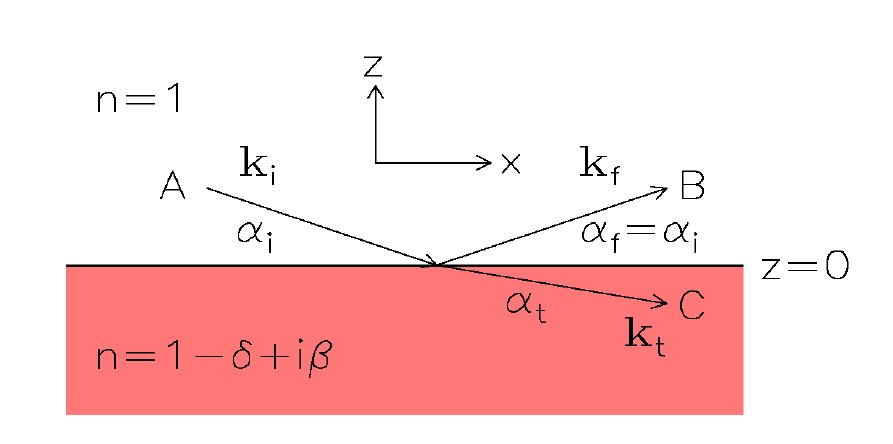
\includegraphics[width=0.8\textwidth]{content/data/reflexion_homogen.jpg}
    \caption{Brechung einer elektromagnetischen Welle auf einer homogenen Schicht.\cite[4]{anleitung_alt}}
    \label{fig:reflexion_homogen}
\end{figure}
\FloatBarrier
Zudem wird die Welle vollständig reflektiert, sobald der Einfallswinkel unter dem kritischen Winkel $\alpha_c$ mit
\begin{equation*}
    \cos \left ( \alpha_c \right ) = n
\end{equation*}
liegt.
Die Absorption liegt in dem Versuch in der Größenordnung $\beta \approx 10^{-7}$ und wird daher vernachlässigt.
Für den kritischen Winkel folgt näherungsweise
\begin{align}
    \alpha_c &\approx \sqrt{2 \delta} \label{eqn:kritisch_exp}\\
    &= \lambda \sqrt{\frac{r_e \rho}{\pi}} \label{eqn:kritisch_th}
\end{align}
, wobei $\lambda$ die Wellenlänge der Röntgenstrahlung, $\rho$ die Elektronendichte des Materials und $r_e$ den Elektronenradius beschreibt.
Der transmittierte und reflektierte Anteil einer senkrecht zur Einfallsebene polarisierten Welle (s-polarisiert) wird durch die Fresnelschen Formeln beschrieben
\begin{align}
    r &= \frac{2 n_1 \cos \left( \alpha_i \right)}{n_1 \cos \left( \alpha_i \right ) + n_2 \cos \left( \alpha_t \right )} \label{eqn:fresnel_r} \\
    t &= \frac{n_1 \cos \left( \alpha_i \right ) - n_2 \cos \left( \alpha_t \right )}{n_1 \cos \left( \alpha_i \right ) + n_2 \cos \left( \alpha_t \right )} \, . \label{eqn:fresnel_t}
\end{align}
Der Transmissions- $t$ und Reflexionskoeffizient $r$ gilt bei Röntgenstrahlung näherungsweise auch für eine t-polarisierte Welle.
\\
Die Intensität einer Welle wird aus dem Betragsquadrat der Feldstärke berechnet. 
Daraus folgt für den Anteil reflektierter Strahlung zur einfallender Strahlung $R = |r^2|$.
Die Fresnelreflektivität $R_F$ kann für Röntgenstrahlung unter der Annahme $\alpha_i > 3 \alpha_c$ zu
\begin{equation}
    R_F \approx \left ( \frac{\alpha_c}{2 \alpha_i} \right )^4
    \label{eqn:fresnelreflektivitaet}
\end{equation}
approximiert werden.
\FloatBarrier

\subsection{Mehrschichtsysteme und der Parratt-Algorithmus}
In diesem Teil wird ein Körper mit \textbf{mehreren Schichten}, statt nur eine glatte Oberfläche betrachtet.
Betrachtet wird ein Polystyrolfilm auf Silizium, das auch in diesem Versuch verwendet wird.
\begin{figure}
    \centering
    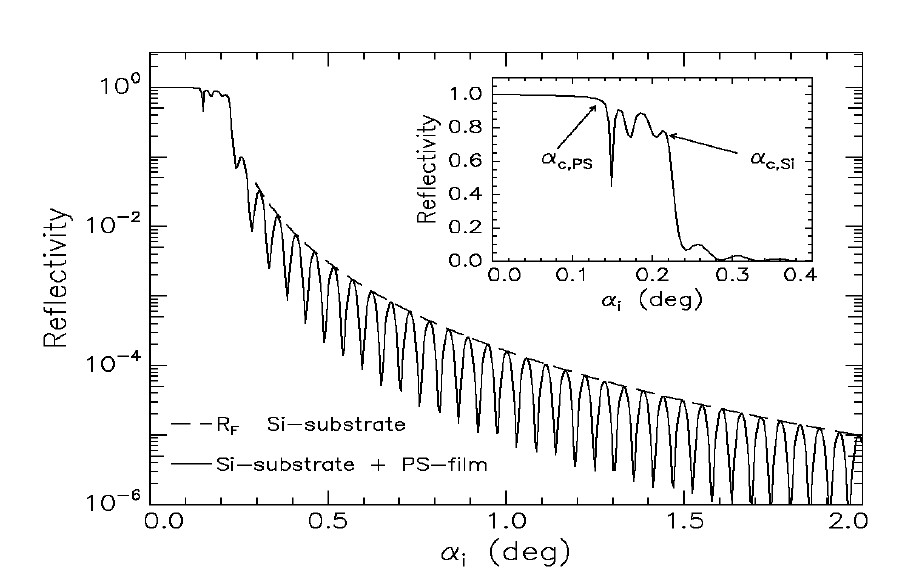
\includegraphics[width=0.8\textwidth]{content/data/reflektivitaet_plot.jpg}
    \caption{Die Reflektivität der Röntgenstrahlung in Abhängigkeit des Einfallswinkels $\alpha_i$.\cite[8]{anleitung_alt}}
    \label{fig:reflektivitaet_plot}
\end{figure}
In \autoref{fig:reflektivitaet_plot} ist die Röntgenreflektiviät in Abhängigkeit des Einfallswinkels $\alpha_i$ aufgetragen.
Der kleine Plot stellt den Bereich bis $\alpha_i = \SI{0.4}{\degree}$ hochauflösend da.
Es existieren zwei Grenzwinkel, der für die Polystyrolschicht $\alpha_\text{c,PS} = \SI{0.15}{\degree}$ und der des Siliziums $\alpha_\text{c,Si} = \SI{0.22}{\degree}$.
Zudem nimmt die Fresnelreflektivität (gestrichelte Linie) bei steigendem Einfallswinkel mit der vierten Potenz, wie nach \autoref{eqn:fresnelreflektivitaet} beschrieben ab.
\\
Die in das Medium eintreffende Welle wird an der Siliziumschicht teils reflektiert und trifft wieder auf das Vakuum und wird reflektiert.
Dieser Prozess wiederholt sich und die Wellen interferieren abhängig von der Phasendifferenz konstruktiv oder destruktiv.
Diese Oszillationen oder Modulationen sind in \autoref{fig:reflektivitaet_plot} zu sehen und werden als "Kiessig-Ringe" bezeichnet.
Beträgt der Gangunterschied $(2n+1) \cdot \frac{\lambda}{2}$ mit $n \in \mathbb{N}$, so kommt es zur destruktiven Interferenz und ein Minimum entsteht.
Ein Interferenzmaximum entsteht hingegen bei geraden Vielfachen von $\frac{\lambda}{2}$.
Die reflektierten Wellen im Medium interferieren konstruktiv miteinander.
\\
Der Schichtabstand bzw. die Dicke der Polystyrolschicht kann nach
\begin{equation}
    d = frac{2\pi}{\Delta q_Z} \approx \frac{\lambda}{2 \Delta \alpha_i}
    \label{eqn:abstand_schicht}
\end{equation}
berechnet werden.
Wobei $\Delta q_Z$ die Differenz der z-Komponente des Wellenvektorübertrags und $\Delta \alpha_i$ die Differenz des Einfallswinkels zwischen zweier Minima darstellt.
\FloatBarrier

Zur Berechnung der Reflektivität in Mehrschichtsystemen wird der rekursiv-arbeitende \textbf{Parratt-Algorithmus} verwendet.